\documentclass{article}
\usepackage[T1]{fontenc}
\usepackage{graphicx}
\usepackage{amsthm}
\usepackage{amsmath}
\usepackage{xcolor}
\usepackage{footnote}
\usepackage{hyperref}
\hypersetup{colorlinks=True,
            linkcolor=brown}
\usepackage{subcaption}
\usepackage{caption}
\usepackage{amssymb}
\usepackage{enumitem}
\usepackage{calrsfs}

\begin{document}

\title{Notes on Recurrent Neural Networks in MLCore}
\author{Solidware}
\date{2 December 2019}
\maketitle


\section{RNN}
\label{rnn}

\subsection{Vanilla RNN}
Although RNN is not used \textit{per se} in MLCore, we start with its definition here, as it introduces more complex architectures that were built on it, like LSTM and GRU, which we used.

The most basic RNN is a single layer neural network. A state vector $s$ is fed from cell to cell, where each cell consists of the application of a non-linearity, $\Phi$ to a given input $x_t$ and previous state $s_{t-1}$ at a given time $t$ ($s_t=0$ at $t$=0):
\begin{equation}
  \label{rnn}
  s_t=\Phi(x_t, s_{t-1}, \Theta)
\end{equation}

with $\Theta$, the parameters of the network to optimise. From there, one can picture an RNN layer in two ways: a "rolled" representation where a single cell is looped over and receives a new observation and state vector at each iteration; or an "unrolled" representation, where each cell is put next to its predecessor and receives the previous state vector and the current observation. Note that since an RNN only has a state vector, $\Theta=\{W_s, U_s, b_s\}$ (first two are referred to as weights, last as bias).

One popular form is the Elman RNN cell defined as: $s_t=\sigma(W_s x_t + U_s s_{t-1} + b_s)$, where $\sigma$ is the sigmoid function; it can also be found written using concatenation formalism $[.;.]$ and a single weight matrix (which it is in practice): $s_t=\sigma(W_s [s_{t-1}; x_t] + b_s)$. An optional (additional) output of the cell would be defined as: $y_t=\Phi(s_t)$ (i.e., $y_t=\sigma(U_y s_t + b_y)$ using additional weight and bias).


Eq.~\ref{rnn} tells something crucial about RNN's behaviour: the state vector of the RNN is fully overwritten at each time step; or put informally, it forgets and replaces everything it just saw since it operates in-place and this dramatically limits the modelling power of such networks. This is known as \textit{information morphing}, for which an RNN cell cannot maintain its prior state completely: even without external input ($x_t$) at time $t$, $s_t=\sigma(a s_{t-1}+b)$ and there exist no $(a,b)$ that allow for an identity mapping between $s_{t-1}$ and $s_t$. This is the root cause of the \textit{degradation problem}\footnote{(He et al., 2015) Deep Residual Learning for Image Recognition (\href{https://arxiv.org/abs/1512.03385}{arXiv:1512.03385}), in which the building block of residual learning can be related to LSTM principles and looks a lot like the state vector update equation ($\mathcal{F}(x,\{W_i\}) \leftrightarrow g_t\textmd{ (in Torch definitions) }$ and $x \leftrightarrow f_t \odot s_{t-1}$)}. Other well-known issues are the \textit{vanishing and exploding gradients}: vanishing does not cause the gradient itself to be small but rather "the gradient's components in directions that correspond to long-term (resp. short-term) dependencies" to be small (resp. larger). In other words, RNNs can easily learn the short-term but not the long-term dependencies; conversely, the \textit{exploding gradient} means long-term dependencies explode to infinity.

\subsection{Details}
Both problems are caused by the RNN's recurring nature: the gradient of the error is essentially equal to the recurrent weight matrix raised to a high power. These iterative matrix powers cause the gradient to grow or to shrink at a rate that is exponential in the number of time steps. A quick explanation (see proof\footnote{(Pascanu et al., 2012) On the difficulty of training recurrent neural networks (\href{https://arxiv.org/abs/1211.5063}{arXiv:1211.5063}) with its own formalism: states ar referred to as $x_{t}$ and inputs as $u_t$.} for details) is given in the following. % of the conditions on singular values of $W$ that cause vanishing/exploding gradients): 

Recall that $s_t=\Phi(W [s_{t-1}; x_t] +b_s)$ and $\widetilde{y_t}=\Phi(V s_t + b_y)$ (the RNN output). Given $\mathcal{E}=\sum_t \mathcal{E}_t$, with $\mathcal{E}_t$ the error (cost) function at time $t$, the goal is to compute the gradient of that error $\mathcal{E}_t(\widetilde{y_t}, y_t)$ wrt. parameters $\Theta=\{W, V, b\}$ and learn good ones using SGD. Knowing that $\frac{\delta\mathcal{E}}{\delta \Theta}=\sum_{1\leq k \leq t} \frac{\delta\mathcal{E}_t}{\delta s_t} \textcolor{green}{\frac{\delta s_t}{s_k}} \frac{\delta s_k}{\delta \Theta}$ by the chain rule, with $\textcolor{green}{\frac{\delta s_t}{s_k}}=\prod_{k \leq i \leq t}\frac{\delta s_i}{s_{i-1}}$, we can understand that it is this product of "$t-k$" Jacobian matrices (which "transports" the errors from time $t$ to time $k$), that can either shrink to 0 or explode to infinity.

It turns out that:
\begin{itemize}[noitemsep,topsep=0pt]
  \item when $\textcolor{red}{\lambda_1 < \frac{1}{\gamma}}$ (where $\gamma=\frac{1}{4}$ if $\Phi$ is a sigmoid (and $\gamma=1$ if $\Phi$ is $tanh$) and
        $\lambda_1$ is the largest singular value of the weight matrix, $W$), the \textcolor{red}{vanishing gradient} occurs and long term contributions will go to 0.
  \item conversely if $\textcolor{blue}{\lambda_1 > \frac{1}{\gamma}}$, long term contributions will \textcolor{blue}{explode}.
  \item note that long-term contributions are those for which $k\ll t$.
\end{itemize}


LSTM were introduced as a solution to the vanishing gradient problem (Pascanu and colleagues proposed another solution in their 2012 paper: regularising gradients to enforce constant backwards error flow). A solution to the exploding gradient problem was also proposed by Pascanu and colleagues (in the same paper), by enforcing a hard constraint over their norm, i.e. shrinking gradients whose norms exceed a threshold (aka gradient clipping\footnote{one may also want to refer to (Mikolov et al., 2014) Learning longer memory in RNN (\href{https://arxiv.org/abs/1412.7753}{arXiv:1412.7753})}). Lastly, one could note that a proper initialisation of weights\footnote{(Glorot and Bengio, 2010) Understanding the difficulty of training deep feedforward neural networks} helps prevent from immediately suffering from these phenomena, but this only impacts the start of the training.


\subsection{LSTM}

\subsubsection{Intuition}
In effect, the original LSTM paper\footnote{(Hochreiter and Schmidhuber, 1997) Long short-term memory} could be reduced to 1 page, and even to 1 paragraph: "Memory cells and gate units" on page 6. That would not be very understandable---hence the other 30 pages (and even with those, that does not make LSTMs a lot clearer)---but the core of the machinery is in there.

Using the analogy of taking notes in a class, a student keeps the information he needs on a paper of paper: he/she doesn't write everything down, nor erases the last sentence every time the professor says something; that process is incremental (additive or substractive: by cherry-picking pieces of information worth writing relative to the original, richer flow of information, or erasing irrelevant details later on). One should therefore remember these 3 natural actions: read, write, forget (as well as the piece of paper, which is the state vector here) because they constitute the 3 gates inside LSTM.

Now put more formally in LSTM, changes to the state vector are incremental, such that $s_{t}\approx s_{t-1} + \Delta s_{t}$ (recall the information morphing problem earlier). A fundamental challenge with those changes is "uncontrolled and uncoordinated writing". Hochreiter and Schmidhuber already recognised this problem and split it into 4 sub-problems, namely: (i) input weight conflict (solution: write selectively), (ii) output weight conflict (solution: read selectively), (iii) abuse problem (solution: forget selectively), and (iv) internal state drift. Solving these conflicts boils down to designing the circuitry of LSTM, but before that, we give more details about each conflict.

\subsubsection{Input weight conflict}
The base RNN writes to every element of the state: $s_t=\Phi(x_t, s_{t-1})$. If each state is written by all units at each time step, it will collect a lot of useless and confusing information, rendering its original state unusable. Hence the new RNN must learn to use some of its units to cancel out some incoming writes and "protect" the state vector (same way I would not write over my last notes, nor write down everything I just heard).

\subsubsection{Output weight conflict}
For each write it makes, the base RNN reads from every element of the state vector. If irrelevant elements are read by all other units at each time step, they produce a potentially huge influx of irrelevant information (overload problem). The new RNN must learn to use some of its units to cancel out irrelevant information.

\subsubsection{Abuse problem}
The issue here is about how to get rid of information that is no longer needed: even if I am selective in writing notes, I would still eventually have no space left (the same way a state vector has finite (lower) dimension), and would otherwise end up writing over important information. The new RNN thus needs a mechanism for selective forgetting in order to make room for new relevant information (i.e., the least relevant older information first needs to be forgotten).

Note that this was not taken care of in the original formulation of LSTMs. (Gers et al., 2000)\footnote{(Gers et al., 2000) Learning to forget: Continual prediction with LSTM} observed that with simple tasks involving long sequences, the state of the original LSTM model would grow indefinitely, eventually causing the network to break down.


\subsubsection{Equations}
\label{eqLSTM}
The three gates mentioned above, namely read/write/forget are vectors of the same size as the state vector and have values between 0 and 1 (this is due to using a sigmoid, which squashes everything into that interval); incidentally, that value can be interpreted as the percentage of reading/writing/forgetting for each state element.

Note that although it is more natural to think of those operations as binary decisions $\{0,1\}$, we need them to be differentiable, hence the choice of the logistic sigmoid function, which produces continuous values between 0 and 1, and is differentiable.

The gates equations\footnote{note that one could rewrite them in a concatenated form, e.g.: $i_t=\sigma(W_i [h_{t-1};x_t ] + b_i)$ for clarity. Additionally, it is possible to define gates' equations using more complex functions; see for example (Wu \textit{et al.}, 2016) On Multiplicative Integration with Recurrent Neural Networks (\href{https://arxiv.org/abs/1606.06630}{arXiv:1606.06630})} of an LSTM are, for $1\leq t \leq L$ (they operate like filters), where $L$ is the sequence length:

\begin{enumerate}[nosep]
  \item $i_t=\sigma(W_{ii}x_t + b_{ii} + W_{hi}h_{t-1} + b_{hi})$, the input gate (write/"save")
  \item $o_t=\sigma(W_{io}x_t + b_{io} + W_{ho}h_{t-1}  + b_{ho})$, the output gate (read/"focus")
  \item $f_t=\sigma(W_{if}x_t + b_{if} + W_{hf}h_{t-1}  + b_{hf})$, the forget gate (forget/"remember")
\end{enumerate}
\medskip

with one extra equation, used to update the cell state:
\begin{enumerate}[resume, nosep]
  \item $j_t = tanh(W_{ij}x_t + b_{ij} + W_{hj}h_{t-1} + b_{hj})$
\end{enumerate}
\medskip

and finally, the states update equations:
\begin{enumerate}[resume, nosep]
  \item $c_t=\textcolor{green}{f_t \odot c_{t-1}} + \textcolor{blue}{i_t \odot j_t}$ (cell state update)
  \item $h_t=\textcolor{red}{o_t \odot tanh(c_{t})}$ (hidden state update)
\end{enumerate}
\medskip

where $(c_t, h_t)$ are the two state vectors (outputs) of LSTM (resp. cell and hidden state), $x_t$ is the input (at time $t$), $W_{i/h.}$ are weight matrices and $b_{i/h.}$ are biases referring respectively to input(i)/hidden(h) and the associated gate.

In a regression problem, $h_{t-1}$ is an estimation of $x_t$. So once the states have been computed at all timesteps $t=1, \dots, L$ (where $L$ may be referred to as the sequence length or window size), we're left with finding a linear mapping between our latent space (which dimension is given by the hidden state vector size) and the output space (which dimension is given by the prediction horizon), i.e. the linear transformation $\widetilde{x}_{L+1} = v^T h_L + b$, where $v$ and $b$ are the weight and bias of the linear function that produces the final prediction result.
% f(x_{t}, \dots, x_{t-T+1}, \textmd{ and any other windowed exogenous obs})


\subsubsection{Summary}
In the original LSTM, "write" comes first: $c_t$ (5.) uses forget (remember) (3.) and input (write) (1.) gates for its update, while $h_t$ (6.) uses the output (read) gate (2.) and $c_t$ (5.). This is somewhat counter-intuitive since we need to read something (the state) in order to be able and write something.

Nevertheless, if creating the "selective write" comes before the read in an RNN cell at time $t$, then that cell must be given a pre-(i.e. $t-1$)-gated hidden state along with the cell state: the \textit{write-then-read} order forces the LSTM to pass both a hidden state and a cell state from one RNN cell to the next. Those stand for:

\begin{itemize}[nosep]
  \item a "slow" state $c_t$ ($c$ for cell or constant error) that fights the vanishing gradient problem and deals with long-term memory via incremental\footnote{(Jozefowicz et al., 2015) An Empirical Exploration of Recurrent Network Architectures} ($+$ or $-$) "selective writes", $\textcolor{blue}{i_t \odot j_t}$ (which fight the input weight conflict) to the gated prior cell states, $\textcolor{green}{f_t \odot c_{t-1}}$ (which fight the abuse problem by "forgetting")
  \item a "fast" state $h_t$ that allows the LSTM to make complex decisions over short periods of time and deals with short-term memory: the "selective reads", $\textcolor{red}{o_t\odot tanh(c_t)}$ of the long-term memory fight the output weight conflict,
\end{itemize}

and have been concatenated in its name: Long Short Term Memory.

\subsection{GRU}
GRU\footnote{(Cho et al., 2014) Learning Phrase Representations using RNN Encoder-Decoder for Statistical Machine Translation (\href{https://arxiv.org/abs/1406.1078}{arXiv:1406.1078}).} are said to be more intuitive (they indeed use only one state, $h$). The gates equations are, for $1\leq t \leq L$ (following pyTorch naming convention):
\begin{enumerate}[nosep]
  \item $\textcolor{blue}{r_t}=\sigma(W_{ir}x_t + b_{ir} + W_{hr} h_{t-1} + b_{hr})$, the update gate
  \item $\textcolor{green}{z_t}=\sigma(W_{iz} x_t + b_{iz} + W_{hz} h_{t-1} + b_{hz})$, the write gate
\end{enumerate}

with one extra equation, used to update the cell state:
\begin{enumerate}[resume, nosep]
  \item $\textcolor{red}{n_t}=\tanh\Big(W_{in} x_t + b_{in} + \textcolor{blue}{r_t} \odot \big( W_{hn} h_{t-1} + b_{hn}\big)\Big) $
\end{enumerate}
\medskip

and finally, the state update equation:
\begin{enumerate}[resume, nosep]
  \item $h_t = (1 - \textcolor{green}{z_t}) \odot \textcolor{red}{n_t} + \textcolor{green}{z_t} \odot h_{t-1}$ (hidden state update)
\end{enumerate}
\medskip

Like LSTM, the final prediction result is available by means of a linear tranformation that maps the latent space to the output space: $\widetilde{x}_{L+1} = v^T h_L + b$.

Differences with LSTM are, in a nutshell:
\begin{itemize}[nosep]
  \item GRUs couple input (1.) and forget (3.) gates into an "update gate", which specifies the proportion of the previous state that we do not want to overwrite.
  \item instead of doing selective forgets and selective writes (in 5.), they use a new "write gate" that is a "$1-$update/forget gate": $h_t=\textcolor{blue}{z_t \odot h_{t-1}} + \textcolor{red}{(1-z_t) \odot j'_t}$, where $z_t$ is the update gate and $j'_t$ is an extra-equation similar to that of LSTM for selective writes (4.), referred to as $n$ in the following.
  \item in other words, everything that is not written is forgotten:
        \begin{itemize}[nosep]
          \item \textcolor{blue}{the first} element-wise product says what not to change/update in the cell state,
          \item \textcolor{red}{the second} does the actual incremental (selective) write where it's allowed to.
        \end{itemize}
  \item GRUs have no peephole connection.
\end{itemize}



\begin{figure}
  \centering
  \begin{subfigure}{0.5\textwidth}
    \centering
    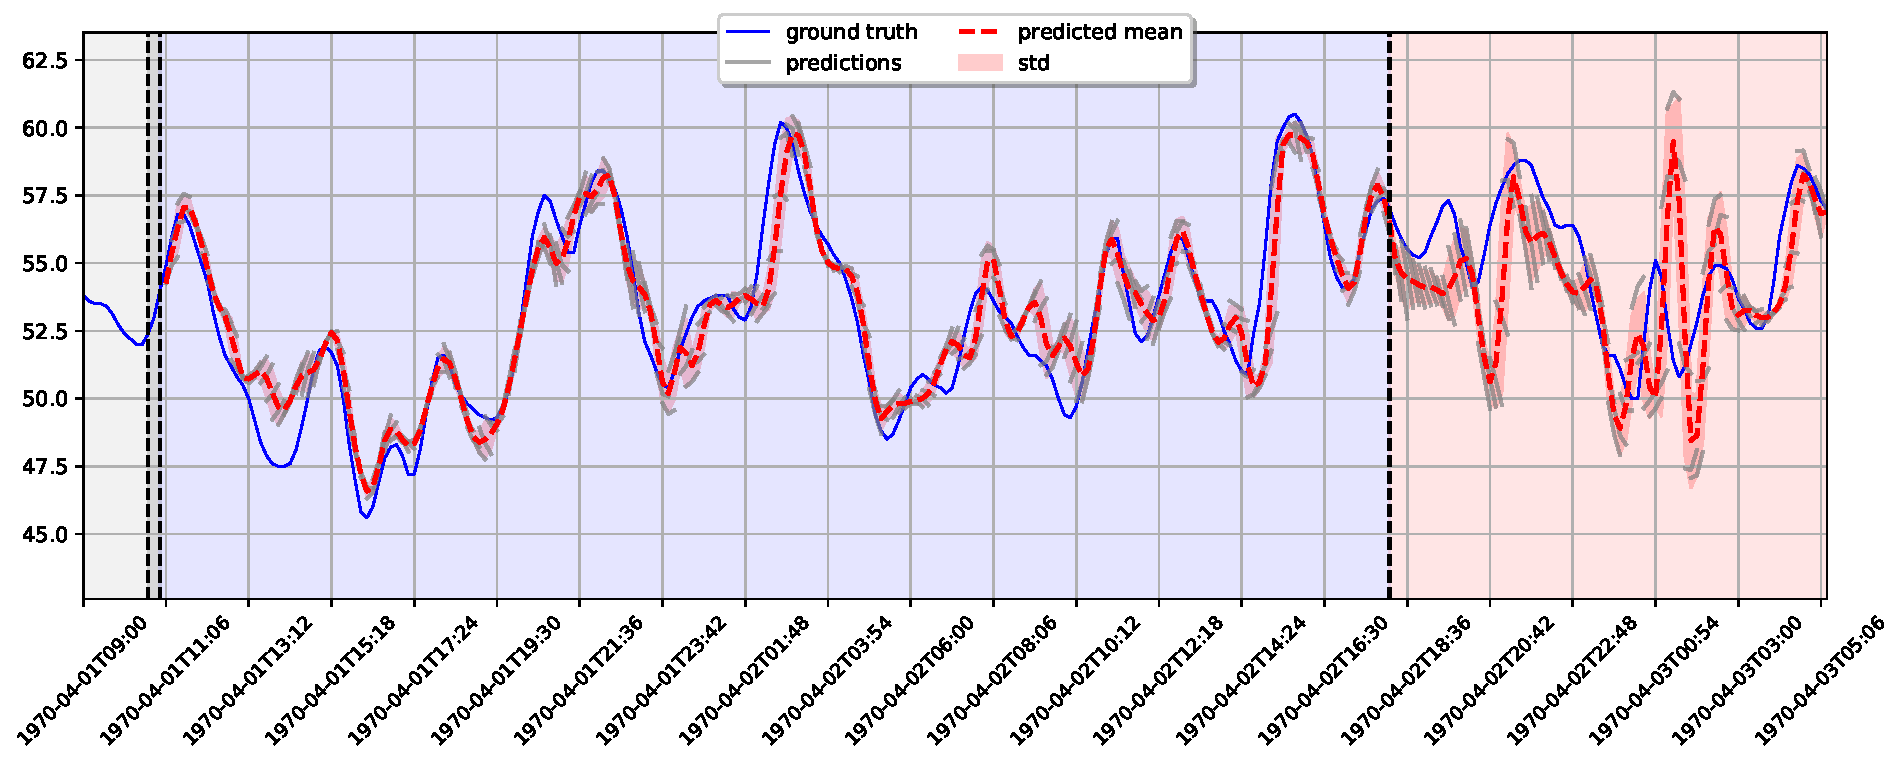
\includegraphics[scale=0.17]{figures/trainCO2_biLSTM_ep120_hs128_nl3_ws12_g2_ph3}
    \caption{}
    \label{fig:fa}
  \end{subfigure}%
  \begin{subfigure}{0.5\textwidth}
    \centering
    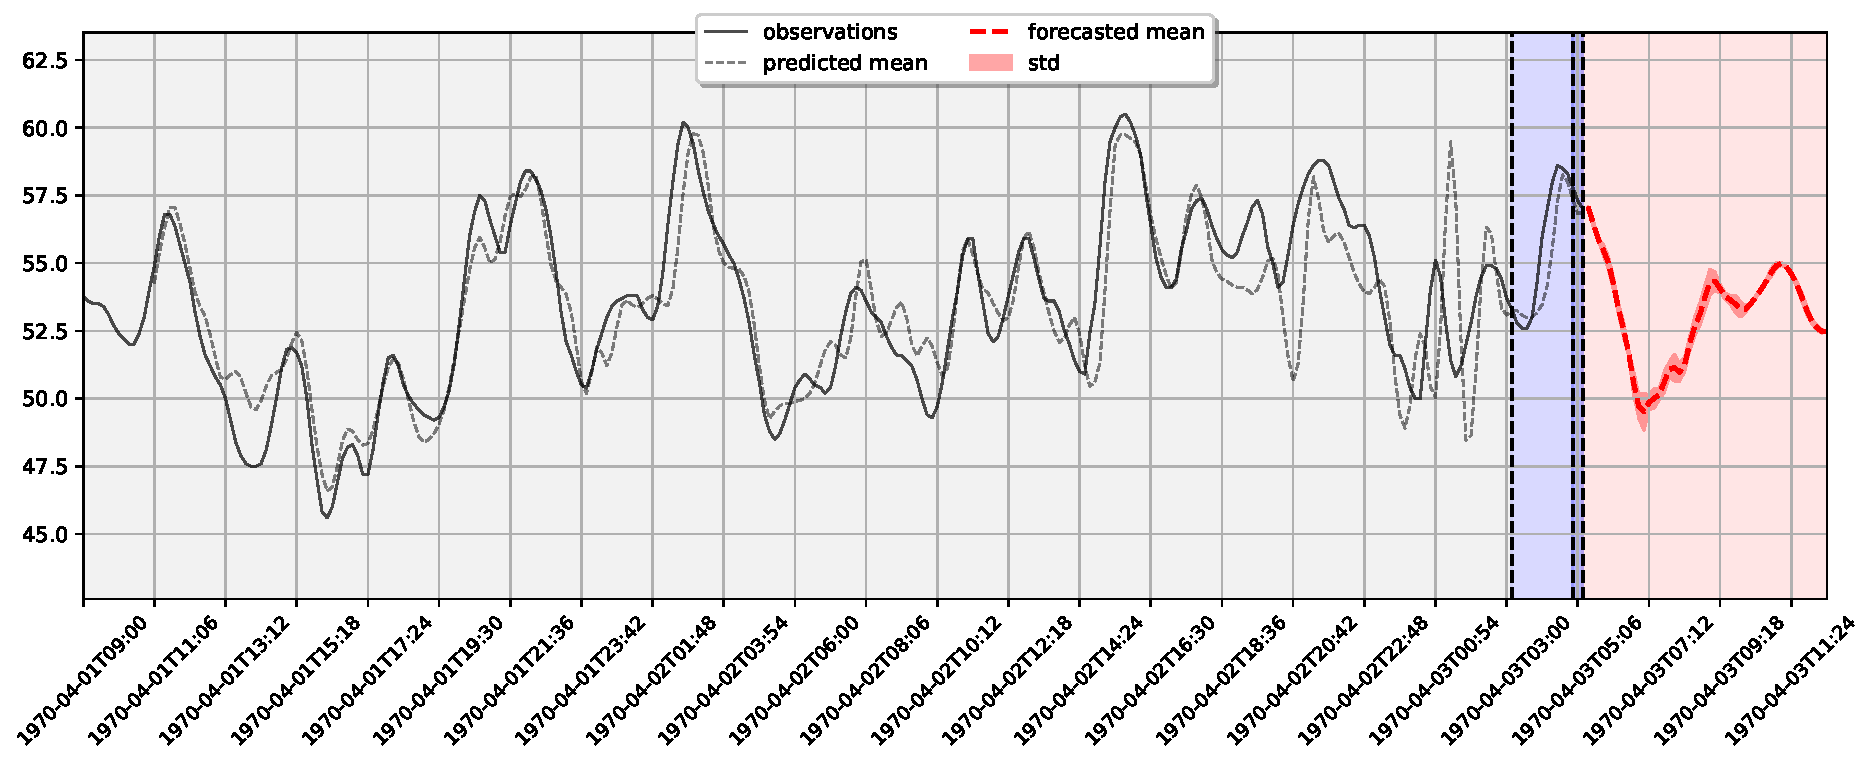
\includegraphics[scale=0.17]{figures/forecastCO2_biLSTM_ep120_hs128_nl3_ws12_g2_ph3}
    \caption{}
    \label{fig:fb}
  \end{subfigure}
  \vspace{3mm}

  \begin{subfigure}{0.5\textwidth}
    \centering
    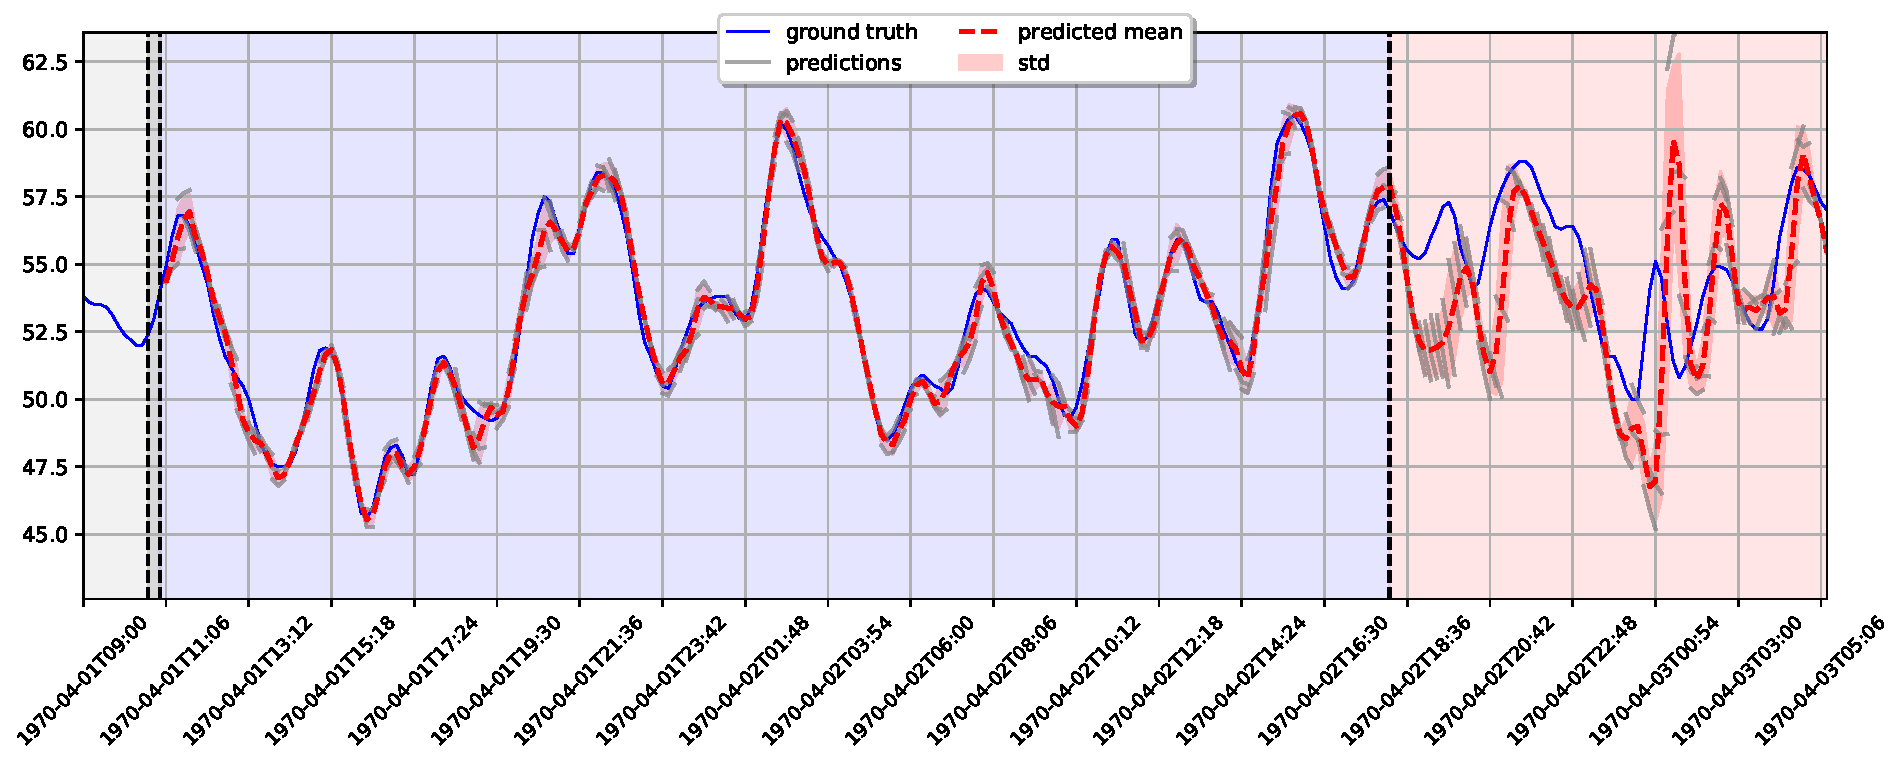
\includegraphics[scale=0.17]{figures/trainCO2_biGRU_ep120_hs128_nl3_ws12_g2_ph3}
    \caption{}
    \label{fig:fc}
  \end{subfigure}%
  \begin{subfigure}{0.5\textwidth}
    \centering
    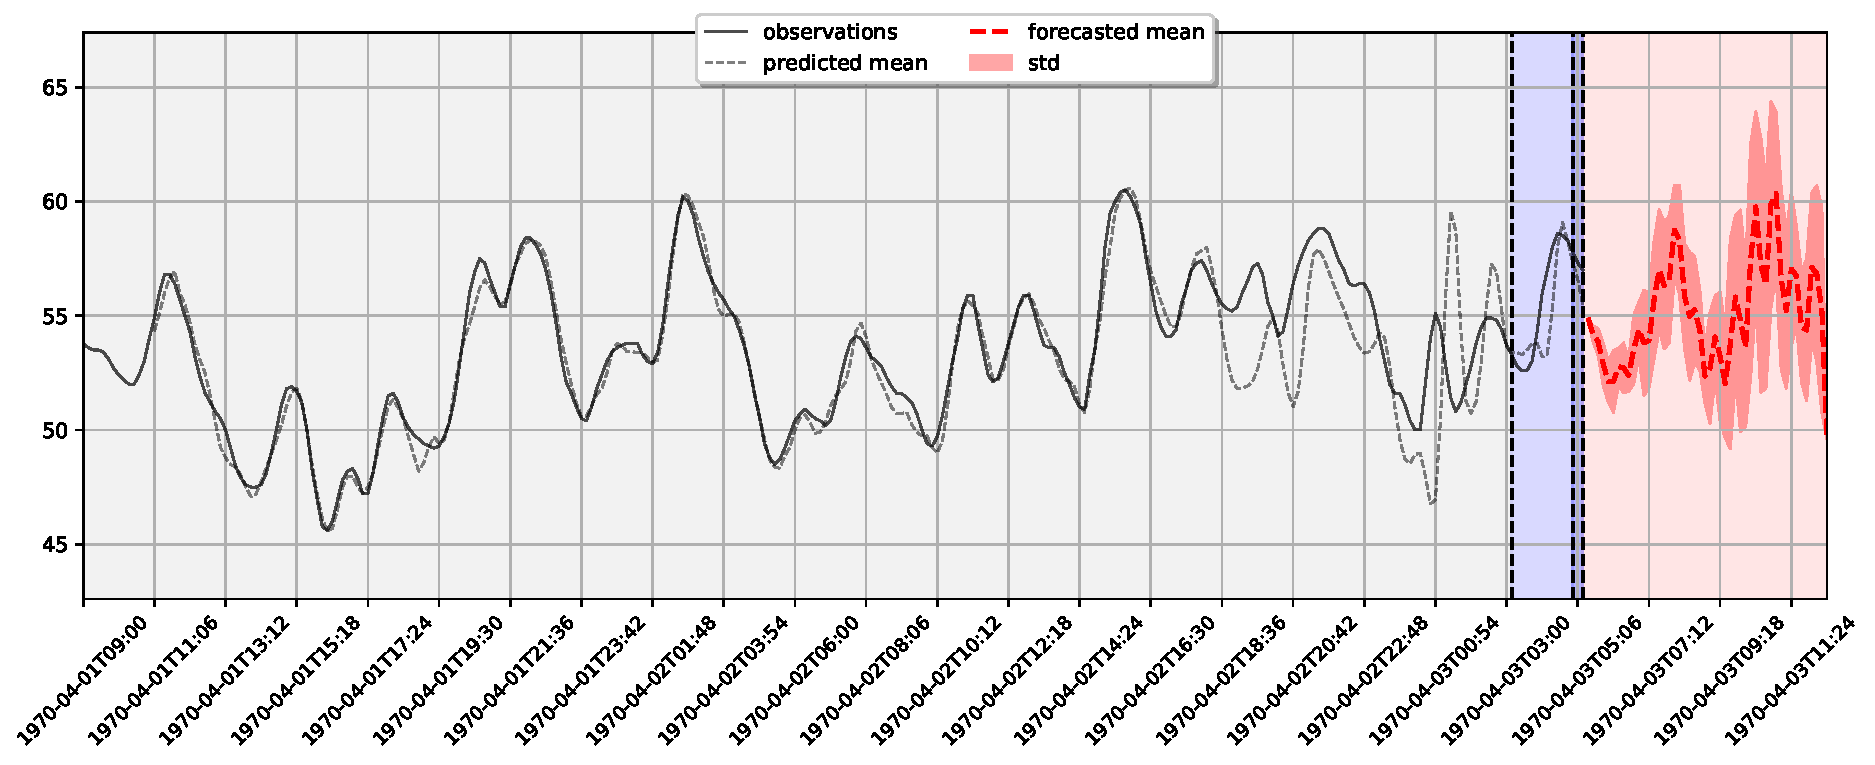
\includegraphics[scale=0.17]{figures/forecastCO2_biGRU_ep120_hs128_nl3_ws12_g2_ph3}
    \caption{}
    \label{fig:fd}
  \end{subfigure}


  \begin{subfigure}{0.5\textwidth}
    \centering
    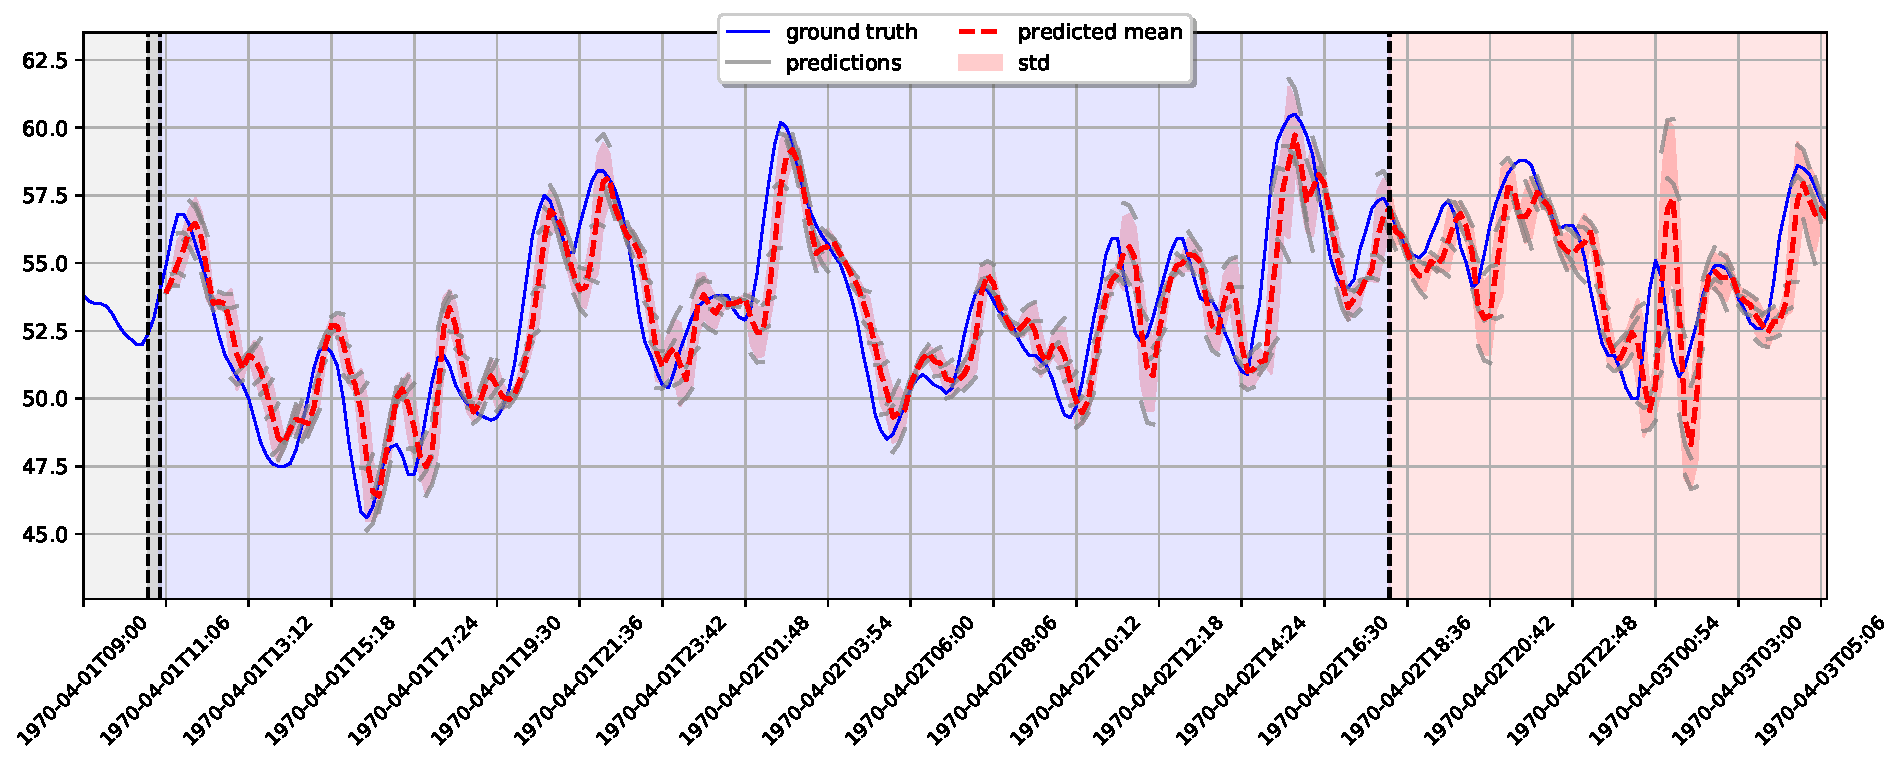
\includegraphics[scale=0.17]{figures/trainCO2_arima_p12_q1_d0_ws12_g2_ph3}
    \caption{}
    \label{fig:fe}
  \end{subfigure}%
  \begin{subfigure}{0.5\textwidth}
    \centering
    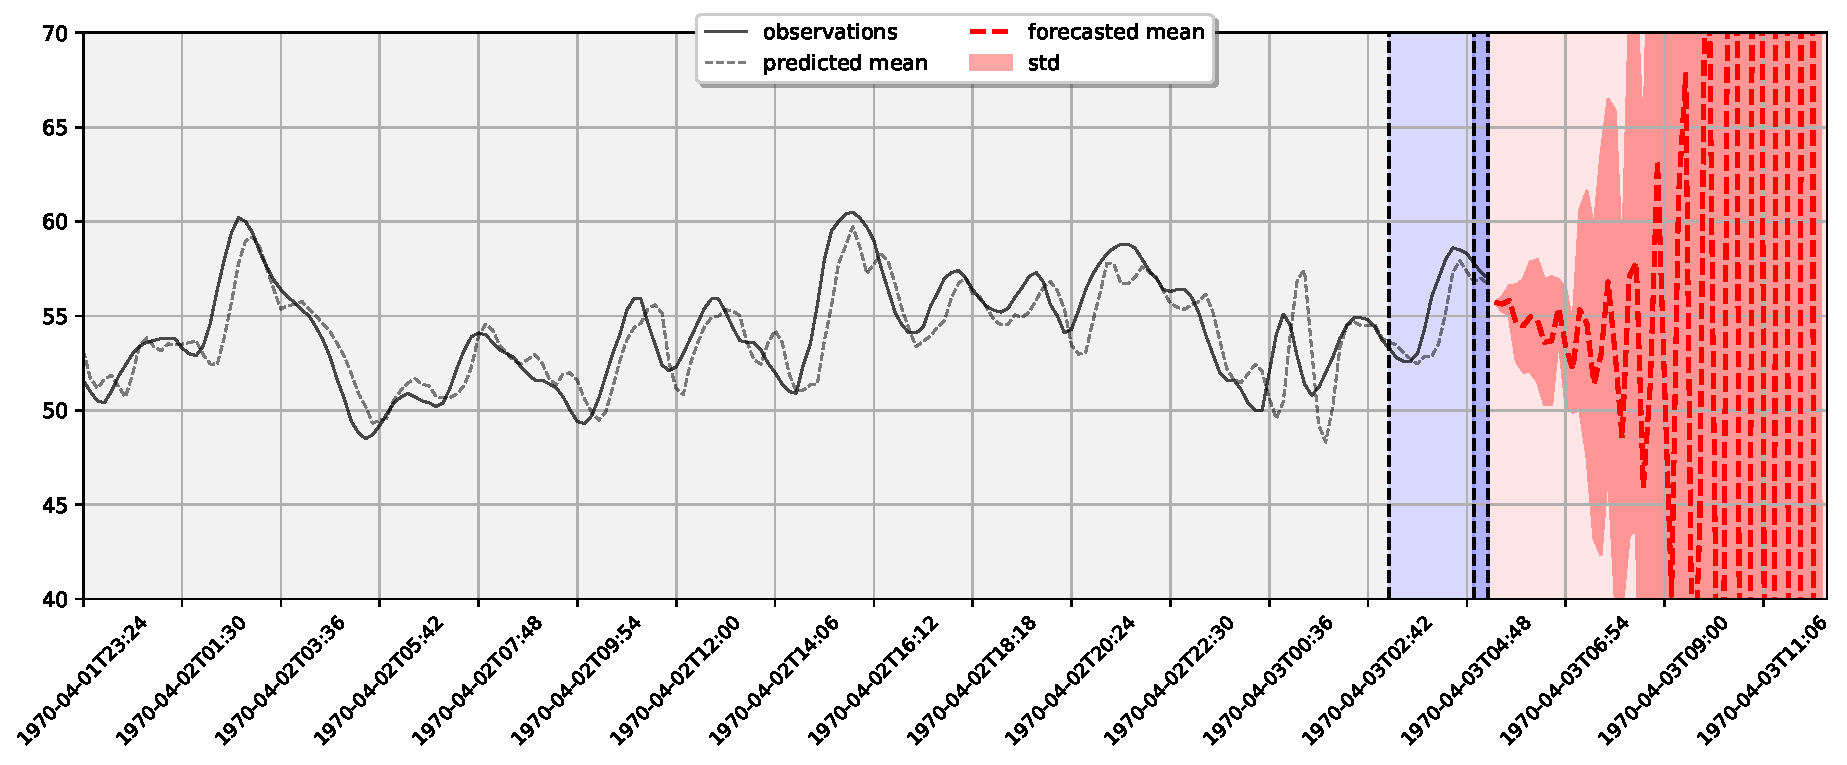
\includegraphics[scale=0.17]{figures/forecastCO2_arima_p12_q1_d0_ws12_g2_ph3}
    \caption{}
    \label{fig:ff}
  \end{subfigure}


  \caption{results on CO2 series using bidirectional LSTM (\ref{fig:fa}) and GRU (\ref{fig:fc}) with L=12, minibatch size=128, 3 layers, hidden size=128, trained over 120 epochs to predict 3 targets ($T+3, T+4, T+5$) with gap=2 and window size=12; forecast is computed recursively up to $T+48$ (\ref{fig:fb}, \ref{fig:fd}). In comparison, ARIMA(12,0,1) behaves like a persistence model on this dataset (\ref{fig:fe}) and forecast diverges (\ref{fig:ff}).}
  \label{fig:fig1}
\end{figure}



\subsection{Results}

Results on methane series (CO2 values) are presented in Fig.~\ref{fig:fig1}

\section{Encoder-decoder architectures}

\subsection{vanilla and seq2seq}
Given an input series $x_t \in \mathbb{R}^n$, and a sequence length $L=4$, we get the trajectory matrix, $X=\mathcal{W}_{L}x_t \in \mathbb{R}^{K\times L}$ where $\mathcal{W}_L$ is the windowing operator of size $L$ and $K=n-L+1$.

An encoder learns a (non-linear) mapping, $f_1$: $s^{(e)}_t=f_1(s^{(e)}_{t-1}, x_t)$ for $1 \leq t \leq L$ with $s^{(e)}_0=(h^{(e)}_0, c^{(e)}_0)=0$, $f_1$ is an LSTM (see Section~\ref{eqLSTM}), and $h^{(e)}_t\in \mathbb{R}^{m}$ (resp. $c^{(e)}_t$), the $m$-long (or $2m$ if the encoder is bidirectional) encoder hidden (resp. cell) state at time step $t$. For future reference (see Section~\ref{attention}), one may be interested in stacking all hidden states at each time step in a matrix, $H\in \mathbb{R}^{L\times m}$ (or $2m$), but for the present case, the decoder is only given the top layer's, latest states, $h^{(e)}_T$ and $c^{(e)}_T$. Recall that a single state is used in GRU.

A decoder learns another mapping (still an LSTM), $f_2$: $s^{(d)}_t=f_2(s^{(d)}_{t-1})$, for $1 \leq t\leq L$ with $s^{(d)}_0=(h^{(e)}_T, c^{(e)}_T)$. It is followed by an output layer with no activation function, which gives: $x_{T+1}=v^T h^{(d)}_T + b$, where $h^{(d)}_T$ is the top layer, latest hidden state of the decoder and $v$, $b$ are the weight and bias of the linear function that produces the final prediction result. Note that the encoder and the decoder are optimised together.

An alternative architecture used e.g. in (Qin et al. 2017) close to seq2seq modeling, consists of letting the encoder give an intermediate lower-dimensional representation of exogenous series (thereby assumed to be available) via the mapping: $f_1$: $s^{(e)}_t=f_1(s^{(e)}_{t-1}, x^{(k)}_t)$, where $x^{(k)}_t$ is now a list of exogenous series values at $t$. The decoder would learn the mapping $f_2$: $s^{(d)}_t=f_2(s^{(d)}_{t-1}, y_t)$, where $y_t$ is the endogenous (target) series values at $t$. A similar linear transformation of $h^{(d)}_T$ would produce the final prediction.



\subsection{Attention}
\label{attention}

\section{Other layers}

\subsection{convolutional RNN}

\subsection{CNN}

\section{Experiments and results}

\end{document}